\documentclass{article}
%\usepackage[a4paper]{geometry}
\usepackage{fullpage}
\usepackage[utf8]{inputenc}
\usepackage[spanish, mexico]{babel}
\usepackage{lipsum}
\usepackage{bm}
\usepackage{upgreek}
\usepackage{enumitem}
\usepackage{mathrsfs}
\usepackage{amsmath}
\usepackage{amssymb}
\usepackage{tikz}
\usepackage{tcolorbox}
\usepackage{csquotes}
\usepackage{helvet}
\usetikzlibrary{arrows, automata}

\tikzset{
    automaton/.style={
        ->, %arrow type
        >=stealth', %arrow head type (bold)
        shorten >=1pt, 
        auto,
        %semithick,
        initial text=$ $, %no start text
    }
}


% mathtools for: Aboxed (put box on last equation in align envirenment)
\usepackage{microtype} %improves the spacing between words and letters

%% COLOR DEFINITIONS

\usepackage{xcolor} % Enabling mixing colors and color's call by 'svgnames'

\definecolor{MyColor1}{rgb}{0.2,0.4,0.6} %mix personal color
\newcommand{\textb}{\color{Black} \usefont{OT1}{lmss}{m}{n}}
\newcommand{\blue}{\color{MyColor1} \usefont{OT1}{lmss}{m}{n}}
\newcommand{\blueb}{\color{MyColor1} \usefont{OT1}{lmss}{b}{n}}
\newcommand{\red}{\color{LightCoral} \usefont{OT1}{lmss}{m}{n}}
\newcommand{\green}{\color{Turquoise} \usefont{OT1}{lmss}{m}{n}}

\DeclareMathOperator{\trace}{trace}
\DeclareMathOperator{\diag}{diag}

%% FONTS AND COLORS

%    SECTIONS

\usepackage{titlesec}
\usepackage{sectsty}
%%%%%%%%%%%%%%%%%%%%%%%%
%set section/subsections HEADINGS font and color
%\sectionfont{\color{Black}}  % sets colour of sections
%\subsectionfont{\color{Black}}  % sets colour of sections

%set section enumerator to arabic number (see footnotes markings alternatives)
\renewcommand\thesection{\arabic{section}} %define sections numbering
\renewcommand\thesubsection{\thesection\arabic{subsection}} %subsec.num.

%define new section style
\newcommand{\mysection}{
\titleformat{\section} [runin] {\usefont{OT1}{lmss}{b}{n}\color{MyColor1}} 
{\thesection} {3pt} {} } 


% %	CAPTIONS
% \usepackage{caption}
% \usepackage{subcaption}
% %%%%%%%%%%%%%%%%%%%%%%%%
% \captionsetup[figure]{labelfont={color=Turquoise}}


%		!!!EQUATION (ARRAY) --> USING ALIGN INSTEAD
%using amsmath package to redefine eq. numeration (1.1, 1.2, ...) 
\renewcommand{\theequation}{\thesection.\arabic{equation}}

\setlength\parindent{0pt}




\makeatletter
\let\reftagform@=\tagform@
\def\tagform@#1{\maketag@@@{(\ignorespaces\textcolor{red}{#1}\unskip\@@italiccorr)}}
\renewcommand{\eqref}[1]{\textup{\reftagform@{\ref{#1}}}}
\makeatother
\usepackage{hyperref}
\hypersetup{colorlinks=true}

% For labeling top of page on every page but first one:
%\usepackage{fancyhdr}

\newcommand{\myclass}{TC1003B -- Modelación de la Ingeniería con Matemática Computacional} % Class name?
\newcommand{\mytitle}{Examen de Módulo} % Title of document?
\newcommand{\mydate}{10.03.2020} % The date?
\newcommand{\myheader}{
    \begin{flushleft}
        \large
        Nombre: \rule{10 cm}{0.4mm} \hfill Matrícula: \rule{2 cm}{0.4mm}\\[1.5ex]
        Nombre: \rule{10 cm}{0.4mm} \hfill Matrícula: \rule{2 cm}{0.4mm}\\[1.5ex]
        Nombre: \rule{10 cm}{0.4mm} \hfill Matrícula: \rule{2 cm}{0.4mm}\\[1.5ex]
        Nombre: \rule{10 cm}{0.4mm} \hfill Matrícula: \rule{2 cm}{0.4mm}
    \end{flushleft}
}

\title{
    \myclass \\
    \textbf{\mytitle} \\
    \myheader
    \date{}
}

% You can set the date automatically by replacing "date goes here" with "\today"

% \renewcommand{\rmdefault}{phv} % Arial Font
\renewcommand{\familydefault}{\sfdefault}

% \pagestyle{fancy}
% \fancyhead{}
% \fancyhead[CO,CE]{{\small{{\bf{\mytitle}} -- \myclass}}}

\newcommand{\responserule}{{\large\rule{14 cm}{0.3mm}}}
\newcommand{\shortresponserule}{{\large\rule{5 cm}{0.3mm}}}
\newcommand{\veryshortresponserule}{{\large\rule{3 cm}{0.3mm}}}

\begin{document}
\maketitle

\vspace{-1.5cm}

{%
\footnotesize
\textit{Lee cuidadosamente y contesta lo que se te pide.
Este examen está pensado para resolverse \textbf{en equipo}, y en poco menos de 90 minutos.
Se sugiere que administres bien tu tiempo.}

\textit{Al momento de contestar, intenten ser lo más explícito posible: se calificará con base en lo que esté escrito, y se considerará el proceso aún cuando la respuesta final esté errada.
Recuerda que puedes revisar material de la clase, el libro de texto o tus notas.
Buena suerte.}
}

\section{Redes Neuronales (100\%)}

Una red neuronal es un mecanismo de aprendizaje automático muy utilizado en inteligencia artificial que sirve para aproximar funciones usando reconocimiento de patrones.
La función que la red neuronal aproxima puede servir para separar en grupos definidos (clasificación) o bien para predecir comportamientos (regresión).

Para entender cómo funciona una red neuronal, primero es necesario entender cómo funciona cada neurona.

\begin{figure}[htbp]
    \centering
    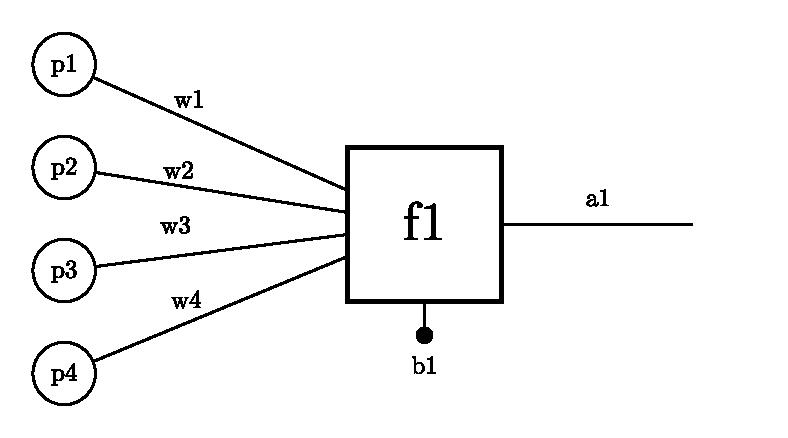
\includegraphics[width=0.7\textwidth]{perceptron.pdf}
    \caption{Perceptrón: una red neuronal de una sola neurona.}
    \label{fig:perceptron}
\end{figure}

Un \textbf{perceptrón} es una red neuronal que consta de una sola neurona, como se muestra en la Figura~\ref{fig:perceptron}.
Una neurona recibe señales por medio de una serie de entradas.
Cada entrada tiene conexiones hacia la neurona, las cuales suelen tener distintos grados de influencia sobre la misma.
Si en conjunto, las señales son lo suficientemente \textit{estimulantes}---a pesar de la predisposición sensorial de la neurona---ésta se activa y \textit{genera} una reacción.
Podemos representar cada uno de sus componentes con símbolos matemáticos:
\begin{itemize}
    \item Un conjunto de \textbf{entradas} o receptores sensoriales $p_j$, donde cada uno representa una característica o variable a tomar en cuenta
    \item Un conjunto de \textbf{pesos} $w_{j}$, donde cada uno determina la importancia que cada entrada ejerce sobre la neurona
    \item Una predisposición sensorial o \textbf{sesgo} $b_i$, que es una cantidad que afecta a la capacidad de la neurona para reaccionar a los estímulos
    \item Una \textbf{función de activación} $f_i$, que genera una reacción a los estímulos que percibe
    \item Una \textbf{salida} o reacción $a_i$, que es generada por la neurona dados los estímulos de sus entradas
\end{itemize}

La suma de cada una de las señales multiplicadas por la influencia que tienen sobre la neurona, más la predisposición sensorial de la misma, es evaluada usando la función de activación de la $i$-ésima neurona para generar una reacción $a_i$:

\begin{equation}
    a_i = f_i\left( \sum_{j=1}^{R} w_jp_j + b_i \right)
\end{equation}

donde $R$ es el número de entradas en la red.

\vspace{2.5ex}

$\blacklozenge$ Contesta para la Figura~\ref{fig:perceptron}:

\begin{itemize}
    \item ¿Cuántas entradas tiene la red? (2 \%)\hfill \veryshortresponserule
    \item ¿Cuántos pesos tiene la red? (2 \%)\hfill \veryshortresponserule
    \item ¿Cuántas neuronas tiene la red? (2 \%)\hfill \veryshortresponserule
    \item ¿Cuántas funciones de activación tiene la red? (2 \%)\hfill \veryshortresponserule
    \item ¿Cuántas salidas tiene la red? (2 \%)\hfill \veryshortresponserule
\end{itemize}

Para hacer el entrenamiento del modelo, el perceptrón toma ejemplos etiquetados---una serie de valores para cada entrada y un resultado esperado.
Tras hacer la evaluación del ejemplo, el resultado obtenido se compara con el resultado esperado, y la diferencia entre ambos se toma como el \textit{error} en la predicción.
Los pesos de la red se ajustan, siempre buscando reducir el error, y se continúa el proceso con otro ejemplo.

Después de unos cuántos (usualmente miles o incluso millones) de ejemplos, el perceptrón aprende un modelo general que trata de aproximar la mayoría de los ejemplos. Sin embargo, existen limitaciones de la arquitectura, y por ello se ha trabajado con arquitecturas más complejas.
Por ejemplo, podemos organizar las neuronas en \textbf{capas}, de tal manera que podemos obtener una serie de reacciones de cada capa en lugar de una sola.

\begin{figure}[htbp]
    \centering
    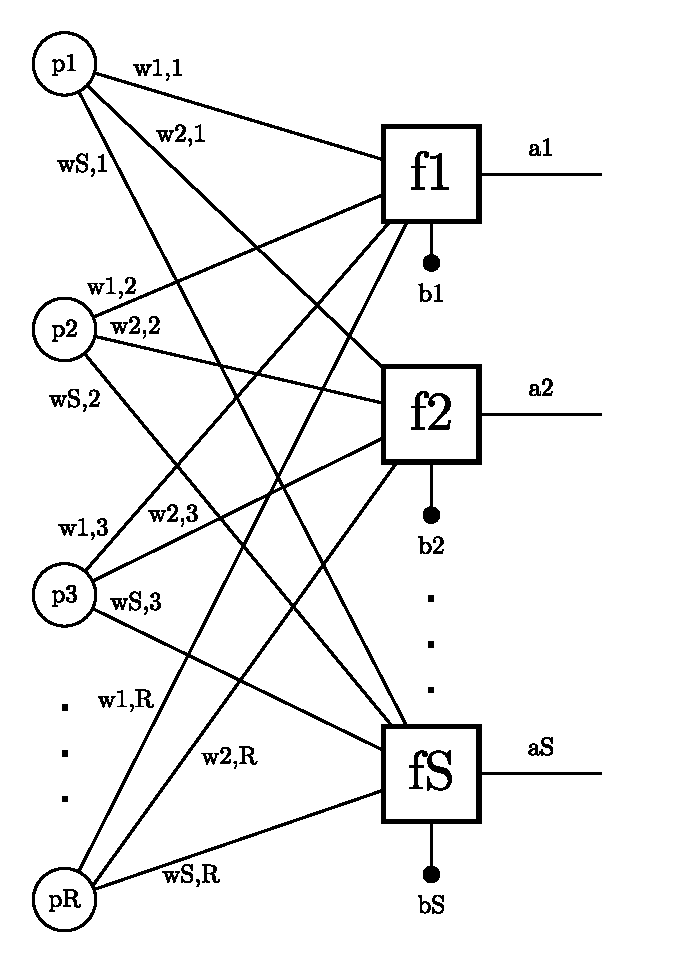
\includegraphics[width=0.8\textwidth]{single-layer-NN.pdf}
    \caption{Red neuronal de una sola capa.}
    \label{fig:single-layer}
\end{figure}

La Figura~\ref{fig:single-layer} ilustra una red neuronal de una sola capa, la cual tiene múltiples entradas y múltiples salidas.
Bajo esta arquitectura, cada entrada $j$ tiene una conexión hacia cada neurona $i$.

\vspace{2.5ex}

$\blacklozenge$ Contesta para la Figura~\ref{fig:single-layer}:

\begin{itemize}
    \item ¿Cuántas entradas tiene la red? (2\%) \hfill \veryshortresponserule
    \item ¿Cuántos pesos tiene la red? (2\%) \hfill \veryshortresponserule
    \item ¿Cuántas neuronas tiene la red? (2\%) \hfill \veryshortresponserule
    \item ¿Cuántas funciones de activación tiene la red? (2\%) \hfill \veryshortresponserule
    \item ¿Cuántas salidas tiene la red? (2\%) \hfill \veryshortresponserule
\end{itemize}

Si te das cuenta, es posible \textit{agrupar} muchas de las variables en juego usando estructuras de datos.

$\blacklozenge$ ¿Qué estructura de datos usarías para representar los componentes de la nueva arquitectura?
Describe la estructura de cada uno (5 \%)

\begin{enumerate}
    \itemsep2.5ex
    \item \responserule
    \item \responserule
    \item \responserule
    \item \responserule
    \item \responserule
\end{enumerate}

Al trabajar todo de manera vectorial, podemos \textit{encadenar} capas para conseguir resultados más finos.

\begin{figure}[htbp]
    \centering
    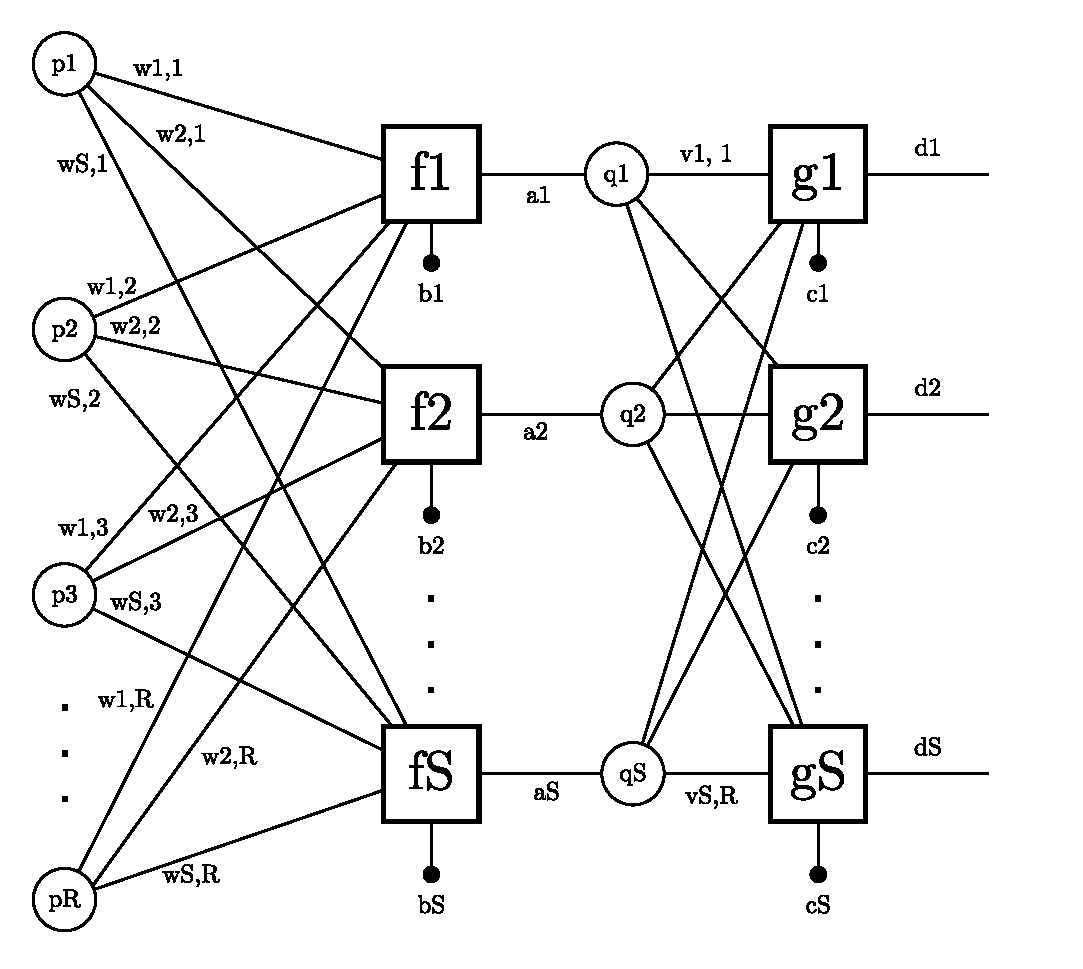
\includegraphics[width=\textwidth]{multi-layer-NN.pdf}
    \caption{Red neuronal de múltiples capas.}
    \label{fig:mlp}
\end{figure}

La Figura~\ref{fig:mlp} ilustra cómo es el proceso de encadenamiento de capas, donde el vector de salidas de una capa es el vector de entradas de la siguiente capa.

En este caso, el proceso de entrenamiento es el mismo, sin embargo las operaciones se pueden simplificar si trabajamos con vectores:

\begin{equation}
    \mathbf{a} = \mathbf{f}\left( W\mathbf{p} + \mathbf{b} \right) = \mathbf{q}
\end{equation}

Vale la pena considerar que una serie de ejemplos $P = \left[ \mathbf{p_i} \dots \mathbf{p}_S \right]$ suele venir en forma matricial, con dimensiones $S \times R$, por lo que para poder multiplicar hay que transponer los ejemplos.

A continuación se presentan algunos ejemplos $\mathbf{p}$ etiquetados con sus resultados $t$ en la forma $P = \mathbf{t}$:

\begin{align}
    3p_1 + 6p_2 - 9p_3 & = 3 \\
    2p_1 + 4p_2 - 8p_3 & = 0 \\
   -2p_1 - 3p_2 + 4p_3 & = -1 \\
    4p_1 + 3p_2 - 7p_3 & = -6 \\
    5p_1 + 4p_2 - 9p_3 & = -7 \\
    7p_1 + 7p_2 - 13p_3 & = -6 \\
   -2p_1 - 5p_2 + 9p_3 & = -2 \\
    -p_1 + 6p_2 + 2p_3 & = 22
\end{align}

$\blacklozenge$ Genera un sistema de ecuaciones lineales usando tres ecuaciones. Para seleccionarlas, utiliza el \textbf{último dígito de tu matrícula}$\mod 8$, enumerando las ecuaciones del 0 al 7 (35 \%)

Considera ahora que tienes una de las siguientes matrices de pesos para la primera capa de una red neuronal con los siguientes datos:

\[
    W^0 = \begin{bmatrix}
        1 & 2 & 2 \\
        2 & 3 & 1 \\
        4 & 2 & 2 \\
        3 & 0 & 2
    \end{bmatrix} \quad W^1=
    \begin{bmatrix}
        2 & 2 & 0 \\
        2 & 1 & 1 \\
        3 & 2 & 2 \\
        5 & 2 & 4 \\
        1 & 2 & 0
    \end{bmatrix}
\]

$\blacklozenge$ Selecciona una de las dos matrices usando tu \textbf{número de equipo} $\mod 2$ y contesta:

\begin{itemize}
    \itemsep2.5ex
    \item ¿Cuál es la longitud del vector de entradas $\mathbf{p}$ de tu matriz? (5 \%)\\ \responserule
    \item ¿Cuántas neuronas tiene la primer capa de la red neuronal que te tocó? (5 \%)\\ \responserule
\end{itemize}

$\blacklozenge$ A continuación, toma la matriz de ejemplos $P$ (Ecuaciones~1.3--1.10) y calcula $P^T$ (5 \%)

\vspace{2.5ex}

$\blacklozenge$ Después, encuentra el vector de salidas de la primera capa ($\mathbf{a}$) considerando que la función de activación de cada neurona en dicha capa de tu red es la función identidad (es decir que $y = x$), y el vector de sesgos $\mathbf{b}$ es o bien
$\mathbf{b^0} = \begin{bmatrix} 1 & 2 & -1 & 1 \end{bmatrix}^T$ o
$\mathbf{b^1} = \begin{bmatrix} -1 & 0  & 0  & 2 & -1 \end{bmatrix}^T$. \textit{\footnotesize Hint: la ecuación 1.2 es de vital importancia} (25 \%)


\section*{Rescate (+5 \%)}

¿Cuál es la principal diferencia entre la descomposición de la matriz de coeficientes entre el método Jacobi y el Gauss-Seidel?

\vfill

\textbf{De acuerdo con el Código de Ética del Tecnológico de Monterrey, mi desempeño en esta actividad estará guiado por la integridad académica.}
\end{document}